%! TEX root = bitirme_tr.tex
%%%%%%%%%%%%%%%%%%%%%%%%%%%%%%%%%%%%%%%%%
% Beamer Presentation
% LaTeX Template
% Version 2.0 (March 8, 2022)
%
% This template originates from:
% https://www.LaTeXTemplates.com
%
% Author:
% Vel (vel@latextemplates.com)
%
% License:
% CC BY-NC-SA 4.0 (https://creativecommons.org/licenses/by-nc-sa/4.0/)
%
%%%%%%%%%%%%%%%%%%%%%%%%%%%%%%%%%%%%%%%%%

%----------------------------------------------------------------------------------------
%	PACKAGES AND OTHER DOCUMENT CONFIGURATIONS
%----------------------------------------------------------------------------------------


\documentclass[
	11pt, % Set the default font size, options include: 8pt, 9pt, 10pt, 11pt, 12pt, 14pt, 17pt, 20pt
	%t, % Uncomment to vertically align all slide content to the top of the slide, rather than the default centered
	%aspectratio=169, % Uncomment to set the aspect ratio to a 16:9 ratio which matches the aspect ratio of 1080p and 4K screens and projectors
]{beamer}

\graphicspath{{Images/}{./}} % Specifies where to look for included images (trailing slash required)
\definecolor{codegreen}{rgb}{0,0.6,0}
\definecolor{codegray}{rgb}{0.5,0.5,0.5}
\definecolor{codepurple}{rgb}{0.58,0,0.82}
\definecolor{backcolour}{rgb}{0.95,0.95,0.92}
\usepackage{listings}
\usepackage{xcolor}
\lstdefinestyle{mystyle}{
    backgroundcolor=\color{backcolour},   
    commentstyle=\color{codegreen},
    keywordstyle=\color{magenta},
    numberstyle=\tiny\color{codegray},
    stringstyle=\color{codepurple},
    basicstyle=\ttfamily\footnotesize,
    breakatwhitespace=false,         
    breaklines=true,                 
    captionpos=b,                    
    keepspaces=true,                 
    numbers=left,                    
    numbersep=5pt,                  
    showspaces=false,                
    showstringspaces=false,
    showtabs=false,                  
    tabsize=2
}

\lstset{style=mystyle}

\usepackage{booktabs} % Allows the use of \toprule, \midrule and \bottomrule for better rules in tables
\usepackage{pgf}
\usepackage{tikz}
\usepackage{llvm/lang}  % include custom language for LLVM IR.
\usepackage{llvm/style}  % include custom style for Nasm
\usetikzlibrary{arrows,shapes,positioning,shadows,trees}
\tikzset{
  basic/.style  = {draw, text width=0.18\textwidth, drop shadow, font=\sffamily, rectangle},
  root/.style   = {basic, rounded corners=2pt, align=center,
                   fill=blue!30},
  level 2/.style = {basic, rounded corners=6pt, thin,align=center, fill=blue!40!green!20},
  level 3/.style = {basic, thin, align=left, fill=blue!10, text width=12.5em}
}

% Define block styles
\tikzstyle{decision} = [diamond, draw, fill=blue!20, 
    text width=4.5em, text badly centered, node distance=3cm, inner sep=0pt]
\tikzstyle{block} = [rectangle, draw, fill=blue!20, 
    text width=3.5em, text centered, rounded corners, minimum height=4em]
\tikzstyle{line} = [draw, -latex']
\tikzstyle{cloud} = [draw, ellipse,fill=red!20, text width=3em, text centered,
    minimum height=4em]
%----------------------------------------------------------------------------------------
%	SELECT LAYOUT THEME
%----------------------------------------------------------------------------------------

% Beamer comes with a number of default layout themes which change the colors and layouts of slides. Below is a list of all themes available, uncomment each in turn to see what they look like.

%\usetheme{default}
%\usetheme{AnnArbor}
%\usetheme{Antibes}
%\usetheme{Bergen}
%\usetheme{Berkeley}
%\usetheme{Berlin}
%\usetheme{Boadilla}
%\usetheme{CambridgeUS}
%\usetheme{Copenhagen}
%\usetheme{Darmstadt}
%\usetheme{Dresden}
%\usetheme{Frankfurt}
%\usetheme{Goettingen}
%\usetheme{Hannover}
%\usetheme{Ilmenau}
%\usetheme{JuanLesPins}
%\usetheme{Luebeck}
\usetheme{Madrid}
%\usetheme{Malmoe}
%\usetheme{Marburg}
%\usetheme{Montpellier}
%\usetheme{PaloAlto}
%\usetheme{Pittsburgh}
%\usetheme{Rochester}
%\usetheme{Singapore}
%\usetheme{Szeged}
%\usetheme{Warsaw}

%----------------------------------------------------------------------------------------
%	SELECT COLOR THEME
%----------------------------------------------------------------------------------------

% Beamer comes with a number of color themes that can be applied to any layout theme to change its colors. Uncomment each of these in turn to see how they change the colors of your selected layout theme.

%\usecolortheme{albatross}
%\usecolortheme{beaver}
%\usecolortheme{beetle}
%\usecolortheme{crane}
%\usecolortheme{dolphin}
%\usecolortheme{dove}
%\usecolortheme{fly}
%\usecolortheme{lily}
%\usecolortheme{monarca}
%\usecolortheme{seagull}
%\usecolortheme{seahorse}
%\usecolortheme{spruce}
%\usecolortheme{whale}
%\usecolortheme{wolverine}

%----------------------------------------------------------------------------------------
%	SELECT FONT THEME & FONTS
%----------------------------------------------------------------------------------------

% Beamer comes with several font themes to easily change the fonts used in various parts of the presentation. Review the comments beside each one to decide if you would like to use it. Note that additional options can be specified for several of these font themes, consult the beamer documentation for more information.

\usefonttheme{default} % Typeset using the default sans serif font
%\usefonttheme{serif} % Typeset using the default serif font (make sure a sans font isn't being set as the default font if you use this option!)
%\usefonttheme{structurebold} % Typeset important structure text (titles, headlines, footlines, sidebar, etc) in bold
%\usefonttheme{structureitalicserif} % Typeset important structure text (titles, headlines, footlines, sidebar, etc) in italic serif
%\usefonttheme{structuresmallcapsserif} % Typeset important structure text (titles, headlines, footlines, sidebar, etc) in small caps serif

%------------------------------------------------

%\usepackage{mathptmx} % Use the Times font for serif text
\usepackage{palatino} % Use the Palatino font for serif text

%\usepackage{helvet} % Use the Helvetica font for sans serif text
\usepackage[default]{opensans} % Use the Open Sans font for sans serif text
%\usepackage[default]{FiraSans} % Use the Fira Sans font for sans serif text
%\usepackage[default]{lato} % Use the Lato font for sans serif text

%----------------------------------------------------------------------------------------
%	SELECT INNER THEME
%----------------------------------------------------------------------------------------

% Inner themes change the styling of internal slide elements, for example: bullet points, blocks, bibliography entries, title pages, theorems, etc. Uncomment each theme in turn to see what changes it makes to your presentation.

%\useinnertheme{default}
\useinnertheme{circles}
%\useinnertheme{rectangles}
%\useinnertheme{rounded}
%\useinnertheme{inmargin}

%----------------------------------------------------------------------------------------
%	SELECT OUTER THEME
%----------------------------------------------------------------------------------------

% Outer themes change the overall layout of slides, such as: header and footer lines, sidebars and slide titles. Uncomment each theme in turn to see what changes it makes to your presentation.

%\useoutertheme{default}
%\useoutertheme{infolines}
%\useoutertheme{miniframes}
%\useoutertheme{smoothbars}
%\useoutertheme{sidebar}
%\useoutertheme{split}
%\useoutertheme{shadow}
%\useoutertheme{tree}
%\useoutertheme{smoothtree}

%\setbeamertemplate{footline} % Uncomment this line to remove the footer line in all slides
%\setbeamertemplate{footline}[page number] % Uncomment this line to replace the footer line in all slides with a simple slide count

%\setbeamertemplate{navigation symbols}{} % Uncomment this line to remove the navigation symbols from the bottom of all slides

\AtBeginSection[]
{
  \begin{frame}
    \frametitle{İçindekiler}
    \tableofcontents[currentsection]
  \end{frame}
}
%----------------------------------------------------------------------------------------
%	PRESENTATION INFORMATION
%----------------------------------------------------------------------------------------

\title[]{RISC-V İşlemcisinin Özel Buyruklarını LLVM Derleyicisiyle Desteklemek} % The short title in the optional parameter appears at the bottom of every slide, the full title in the main parameter is only on the title page

%\subtitle{Optional Subtitle} % Presentation subtitle, remove this command if a subtitle isn't required

\author[]{Mehmet Eymen Ünay \\ 504231201 } % Presenter name(s), the optional parameter can contain a shortened version to appear on the bottom of every slide, while the main parameter will appear on the title slide

\institute[]{İstanbul Teknik Üniversitesi \\ \smallskip Elektronik Mühendisliği} % Your institution, the optional parameter can be used for the institution shorthand and will appear on the bottom of every slide after author names, while the required parameter is used on the title slide and can include your email address or additional information on separate lines

\date[\today]{} % Presentation date or conference/meeting name, the optional parameter can contain a shortened version to appear on the bottom of every slide, while the required parameter value is output to the title slide


%----------------------------------------------------------------------------------------

\begin{document}

%----------------------------------------------------------------------------------------
%	TITLE SLIDE
%----------------------------------------------------------------------------------------

\begin{frame}
	\titlepage % Output the title slide, automatically created using the text entered in the PRESENTATION INFORMATION block above
\end{frame}
%----------------------------------------------------------------------------------------
%	TABLE OF CONTENTS SLIDE
%----------------------------------------------------------------------------------------

% The table of contents outputs the sections and subsections that appear in your presentation, specified with the standard \section and \subsection commands. You may either display all sections and subsections on one slide with \tableofcontents, or display each section at a time on subsequent slides with \tableofcontents[pausesections]. The latter is useful if you want to step through each section and mention what you will discuss.

\begin{frame}
	\frametitle{Sunum Planı} % Slide title, remove this command for no title
	
	\tableofcontents % Output the table of contents (all sections on one slide)
	%\tableofcontents[pausesections] % Output the table of contents (break sections up across separate slides)
\end{frame}

%----------------------------------------------------------------------------------------
%	PRESENTATION BODY SLIDES
%----------------------------------------------------------------------------------------

\section{Introduction}
\begin{frame}{Giriş}
\begin{itemize}
        \item Programlama dilleri ve derleyicileri, yaygın mimariler için geliştirilmiştir.
        \item Standart ISA'yı (Buyruk Kümesi Mimarisi) hedefleyen bir derleyici, özel donanım için özel buyruklar üretmeyecektir.
	\item Özel donanımı yüksek seviyeli dillere tanıtmak için derleyici modifikasyonuna ihtiyaç vardır.
	\item Bu projede, LLVM ile özel talimatları destekleyerek bu sorunu çözmeyi hedefledik.
    \end{itemize}

\end{frame}

\section{Derleyici Yapısı} % Sections are added in order to organize your presentation into discrete blocks, all sections and subsections are automatically output to the table of contents as an overview of the talk but NOT output in the presentation as separate slides

%------------------------------------------------

\begin{frame}{Derleyici Yapısı}
Bir derleyicinin farklı aşamaları vardır, ancak “Ön Uç (Front-End)” ve “Arka Uç (Back-End)” olmak üzere iki ana bölüme gruplandırılabilirler
	\begin {itemize}
	    \item Leksikal Analiz (Lexical Analysis)
	    \item Sözdizimi Analizi (Syntax Analysis)
	    \item Semantik Analiz 
	    \item Ara Kod Üretimi (Intermediate Representation)
	    \item Kod Optimizasyonu
	    \item Hedef Kod Üretimi (Target Code)	    
	\end {itemize}	
\end{frame}


\section{LLVM Yapısı} % Sections are added in order to organize your presentation into discrete blocks, all sections and subsections are automatically output to the table of contents as an overview of the talk but NOT output in the presentation as separate slides

%------------------------------------------------
\subsection{LLVM Derleyicisi}
\begin{frame}{LLVM Nedir?}
	\begin {itemize}
	    \item LLVM bir derleyici altyapısıdır.
	    \item Modüler ve yeniden kullanılabilir derleyici ve araç zinciri teknolojilerinin bir koleksiyonudur.
        \item 3000 katılımcı ile 450.000'den fazla kod commit'i.
	\end {itemize}
\end{frame}
\begin{frame}{Genel Yapı}
    \begin{figure}
	   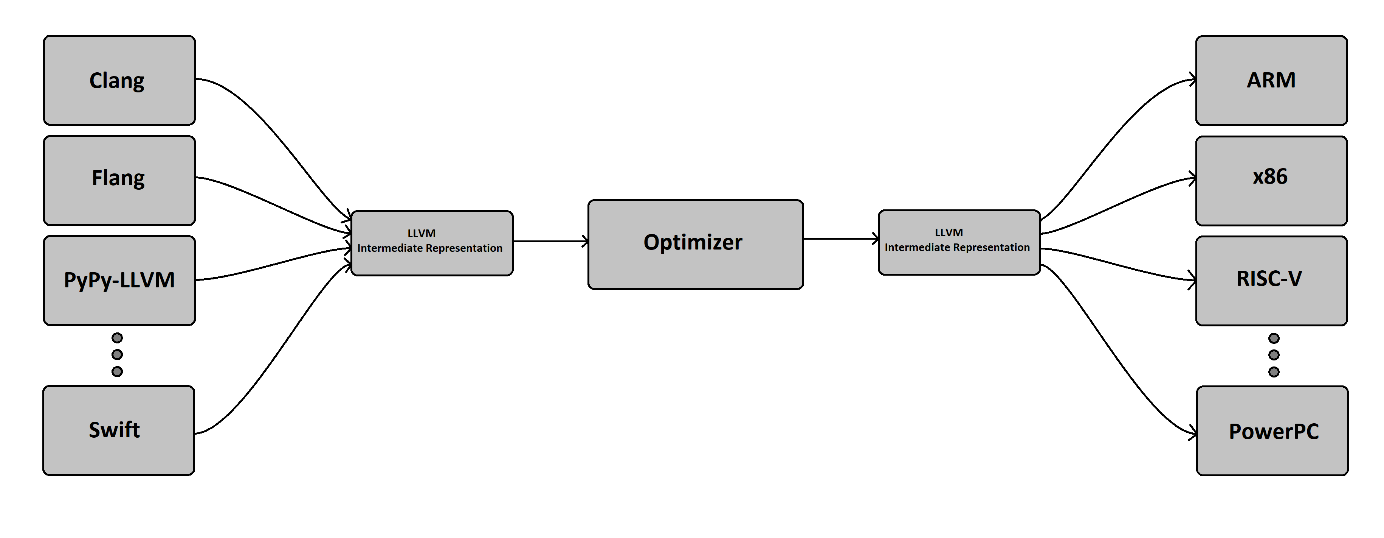
\includegraphics[width=0.8\linewidth]{llvm_diagram.png}
	   \caption{LLVM Frontend ve Backend}
	\end{figure}
\end{frame}

\subsection{LLVM Derleyicisi Backend}
\begin{frame}{Backend}
    \begin{itemize}
        \item Talimat Seçimi (Instruction Selection)
        \item Zamanlama ve Oluşturma
        \item SSA tabanlı Makine Kodu Optimizasyonları
        \item Yazmaç Atama (Register Allocation)
        \item Prolog/Epilog Kodu Ekleme
        \item Kod Yayımı
        \item Bağlama (Linking)
        
    \end{itemize}
\end{frame}

\begin{frame}{Talimat Seçimi Çerçeveleri}
    \begin{itemize}
        \item FastISel
        \item SelectionDAG
        \item GlobalISel
    \end{itemize}
\end{frame}

\begin{frame}{SelectionDAG}
    \begin{enumerate}
    \item 
    İlk DAG'ı Oluştur
    \item
    SelectionDAG'ı Optimize Et
    \item
    SelectionDAG Türlerini Yasallaştır (Legalize Types)
    \item
    SelectionDAG'ı Optimize Et 
    \item
    SelectionDAG İşlemlerini Yasallaştır (Legalize Ops)
    \item
    SelectionDAG'ı Optimize Et
    \item
    DAG'dan talimatları seç
    \item
    SelectionDAG Zamanlama ve Oluşturma
    \end{enumerate}

	\begin{definition}
		\alert{Yönlü Çevrimsiz Grafik (DAG)}, çevrimi olmayan yönlü bir graf'tır.
	\end{definition}
\end{frame}

\section{C'den Assembly'ye Yol}
\begin{frame}{Hedef Düşürme Adımları}
    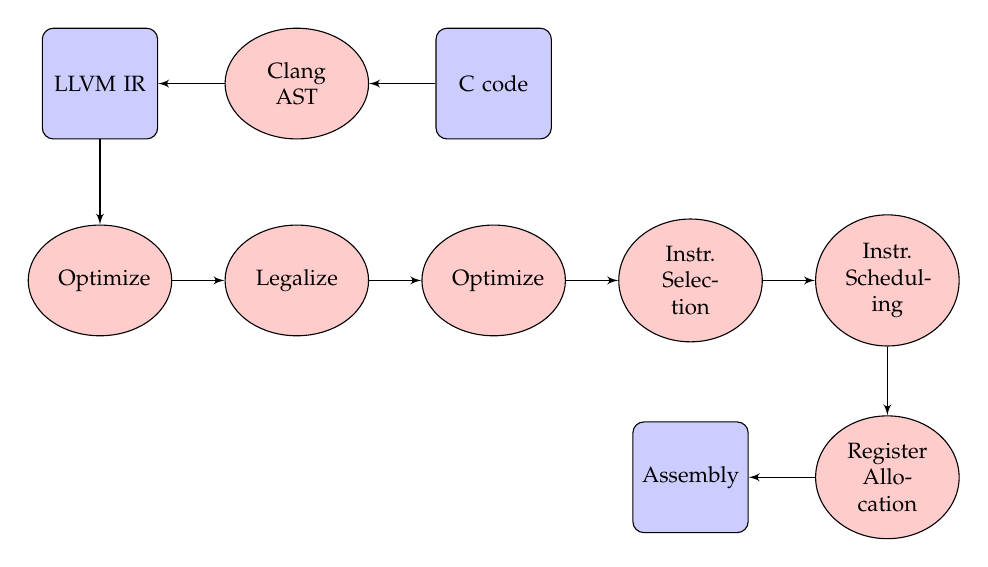
\begin{tikzpicture}[node distance = 2cm, auto]
\centering
\tikzstyle{every node}=[font=\footnotesize]
    % Place nodes
    \node [block] (init) {C code};
    \node [cloud, left of=init,node distance=2.5cm] (ast) {Clang AST};
    \node [block, left of=ast,node distance=2.5cm] (llvmir) {LLVM IR};
    \node [cloud, below of=llvmir,node distance=2.5cm] (opt1) {Optimize};
    \node [cloud, right of=opt1,node distance=2.5cm] (leg) {Legalize};
    \node [cloud, right of=leg,node distance=2.5cm] (opt2) {Optimize};
    \node [cloud, right of=opt2,node distance=2.5cm] (sel) {Instr. Selection};
    \node [cloud, right of=sel,node distance=2.5cm] (sched) {Instr. Scheduling};
    \node [cloud, below of=sched,node distance=2.5cm] (reg) {Register Allocation};
    \node [block, left of=reg,node distance=2.5cm] (assem) {Assembly};

    % Draw edges
    \path [line] (init) -- (ast);
    \path [line] (ast) -- (llvmir);
    \path [line] (llvmir) -- (opt1);
    \path [line] (opt1) -- (leg);
    \path [line] (leg) -- (opt2);
    \path [line] (opt2) -- (sel);
    \path [line] (sel) -- (sched);
    \path [line] (sched) -- (reg);
    \path [line] (reg) -- (assem);
   
\end{tikzpicture}
\end{frame}

\begin{frame}[fragile]{Örnek C Kodu}
\begin{lstlisting}[language=C]
int a,b,c;
void maddFunc() {
	a = 3;
	b = 103;
	c = 127;
	a = a * b + c;
}
\end{lstlisting}
\end{frame}

\begin{frame}[fragile]{LLVM IR}
\lstinputlisting[caption={LLVM IR generated by Clang},label={fig:llvm_ir}, language=llvm, style=nasm]{../thesis/path_instruction/madd.ll}
\end{frame}


\begin{frame}{Yasallaştırmadan ve Optimizasyonlardan Sonra DAG}
    \begin{figure}
    \centering
    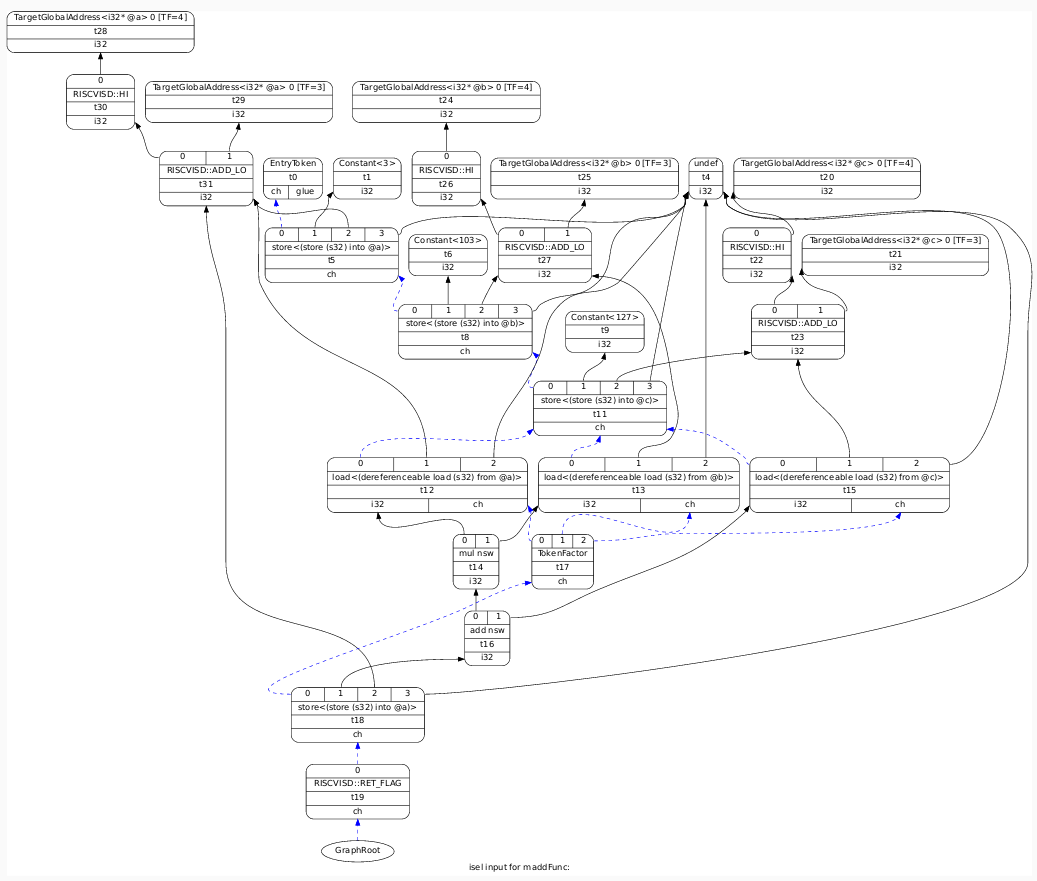
\includegraphics[height=0.75\textheight]{path_instruction/madd_dag_isel.png}
    \caption{Talimat Seçiminden Önce DAG}
    \label{fig:isel}
\end{figure}
\end{frame}

\begin{frame}{Talimat Seçiminden Sonra DAG}
    \begin{figure}
    \centering
    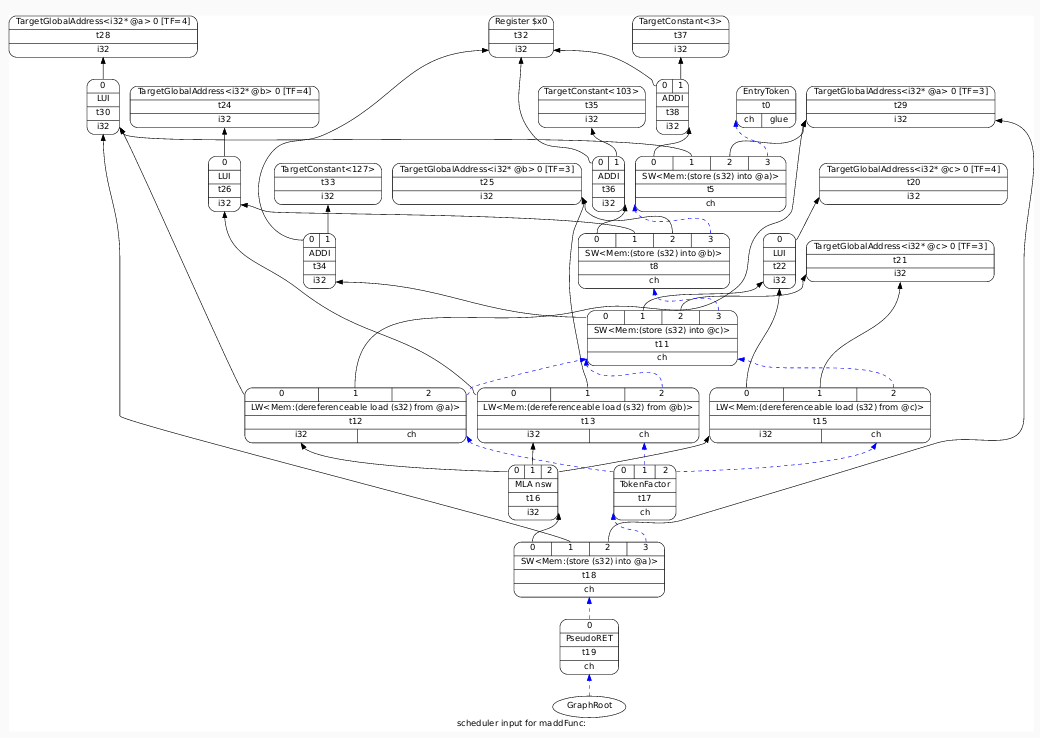
\includegraphics[height=0.75\textheight]{path_instruction/madd_dag_sched.png}
    \caption{DAG after Instruction Selection}
    \label{fig:dag_sched}
\end{figure}
\end{frame}


\begin{frame}[fragile]{Final Assembly}
    \begin{lstlisting}[ caption=madd.s Assembly Output]
    ...
	lui	a0, %hi(a)
	li	a1, 3
	sw	a1, %lo(a)(a0)
	lui	a1, %hi(b)
	li	a2, 103
	sw	a2, %lo(b)(a1)
	lui	a2, %hi(c)
	li	a3, 127
	sw	a3, %lo(c)(a2)
	lw	a3, %lo(a)(a0)
	lw	a1, %lo(b)(a1)
	lw	a2, %lo(c)(a2)
	mla	a1, a3, a1 ,a2
	sw	a1, %lo(a)(a0)
	lw	ra, 12(sp)     
	lw	s0, 8(sp)      
    ...
	ret
\end{lstlisting}
\end{frame}

\section{SelectionDAG'de RISC-V Tanımı}
\subsection{TableGen Kayıt Bildirimi}
\begin{frame}{TableGen}
    \begin{itemize}
        \item LLVM arka uç tarafında CPP başlık (header) dosyaları oluşturmak için kullanılan alan-özel dili. (Domain specific language/DSL)
        \item
        Talimat bildirim kodundaki fazlalıkları kaldırır
        \item
        Sınıflar, ortak bilgileri aktarmak için kullanılır ve kayıtlara (Records) miras kalır
        \item
        Komutsal (Imperative) yerine Bildirimsel (Declarative)
    \end{itemize}
\end{frame}

\begin{frame}[fragile]{RISC-V TableGen Sınıfları}
Hedef Bağımsız Talimat Sınıfları
    \begin{itemize}
        \item \textbf{InstructionEncoding}, çözücü metodu, talimatın boyutu
        \item
        \textbf{Instruction}, giriş ve çıkış DAG'ları
    \end{itemize}

'XOR' Talimatını bildirmek için Miras Alınan RISC-V Talimat Sınıfları
    \begin{itemize}
        \item \textbf{RVInst}, RISC-V'ın evrensel bit desenleri
        \item
        \textbf{RVInstR}, R tipi talimat
        \item
        \textbf{ALU\_rr}, değişme özelliği (commutativity) gibi özellikler bildirildi
    \end{itemize}
\begin{lstlisting}
def XOR  : ALU_rr<0b0000000, 0b100, "xor", /*Degisebilir*/1>,
           Sched<[WriteIALU, ReadIALU, ReadIALU]>;
\end{lstlisting}
\end{frame}


\subsection{TableGen Desen Eşleştirme}
\begin{frame}[fragile]{TableGen Desenleri}
RISC-V TableGen sınıfları, herhangi bir talimatı daha yapılandırılmış bir şekilde bildirmek için kullanılabilir.
\par
Talimatın DAG deseni, TableGen'in bir Desen bildiriminde ilan edilebilir. NAXOR (NOT AND XOR) talimatı için bu: LLVM IR montaj (assembly) talimatları ve içsel fonksiyonlar (intrinsic functions) DAG yapısında birleştirilir.

\begin{lstlisting}
def : Pat< (xor (and (not GPR:$src1), GPR:$src2), GPR:$src3),
(NAXOR GPR:$src1, GPR:$src2, GPR:$src3)>;
\end{lstlisting}
\end{frame}

        

\begin{frame}[fragile]{TableGen Desenleri}
\begin{lstlisting}
let hasSideEffects = 0, mayLoad = 0, mayStore = 0 in
class ALU_rrr<bits<2> funct2, bits<3> funct3, string opcodestr,
             bit Commutable = 0>
    : RVInstR4<funct2, funct3, OPC_OP, (outs GPR:$rd), (ins GPR:$rs1, GPR:$rs2, GPR:$rs3),
              opcodestr, "$rd, $rs1, $rs2 ,$rs3"> {
  let isCommutable = Commutable;
}
\end{lstlisting}
ALU\_rrr adında özel bir talimat sınıfı oluşturuldu. NAXOR talimatı üç kaynak yazmaç gerektirir ve ALU türü olarak tanımlanır. 
\end{frame}


        
\begin{frame}[fragile]{TableGen Desenleri}
\begin{lstlisting}
def NAXOR     : ALU_rrr<0b11, 0b100, "naxor">,
Sched<[WriteIMul, ReadIMul, ReadIMul]>;
\end{lstlisting}
NAXOR talimatı tanımlanmıştır ve ALU\_rrr talimat türü kullanılmıştır. funct2, funct3, opcode dizesi ve programlar, özel ALU\_rrr sınıfı sayesinde talimatın tam tanımına sahip olmak için yeterlidir.
\end{frame}



\begin{frame}[fragile]{TableGen Desenleri}
\begin{figure}
    \centering
    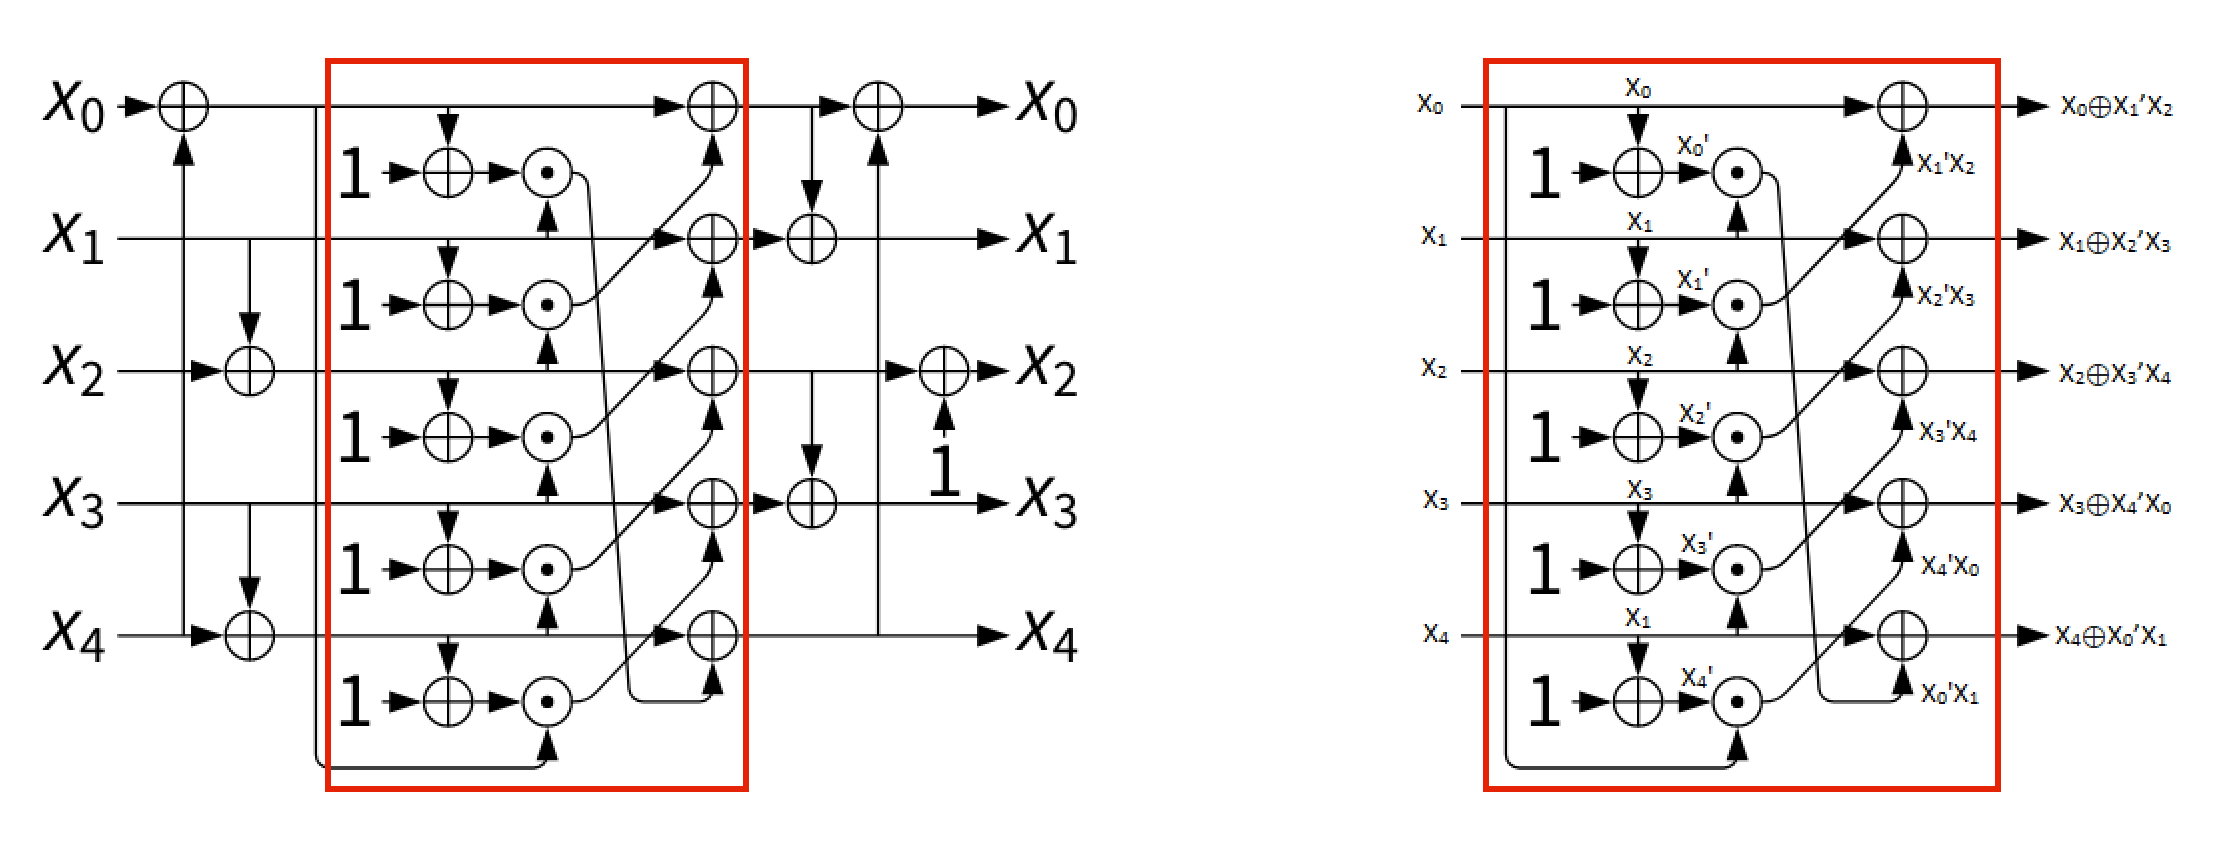
\includegraphics[scale=0.15]{sbox_naxor_pattern.png}
    \caption{NAXOR desenleri s-box algoritmasında}
    \label{fig:sbox_naxor_pattern}
\end{figure}
Bu desen, Şekil \ref{fig:sbox_naxor_pattern}'de vurgulandığı gibi 5 kez tekrarlanır. NAXOR talimatı 15 talimatı 5 talimata indirger.
\end{frame}



\begin{frame}[fragile]{TableGen Desenleri}
\begin{figure}
    \centering
    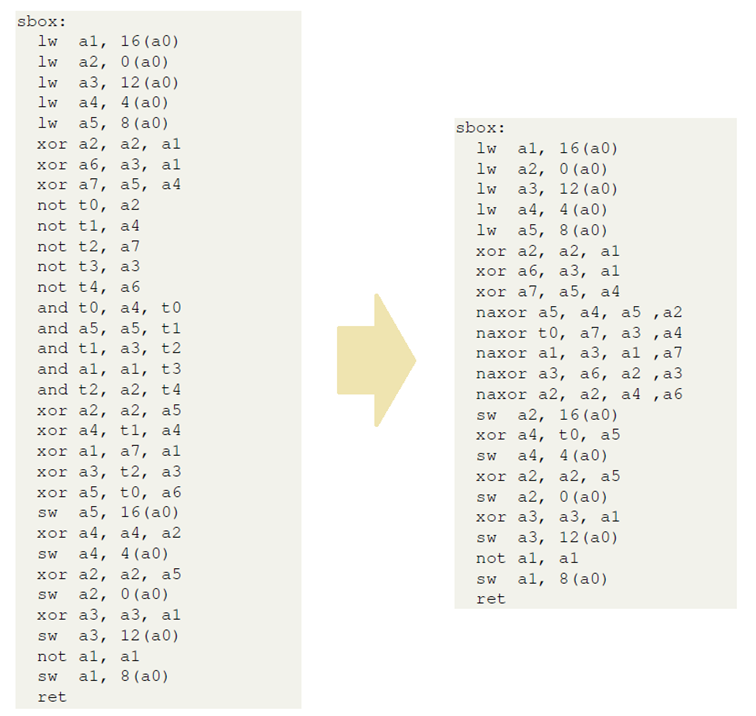
\includegraphics[scale=0.27]{naxor_instruction.png}
    \caption{NAXOR talimatının S-BOX montaj kodu üzerindeki etkisi}
    \label{fig:sbox_instruction}
\end{figure}
S-box algoritması, tekrar tekrar kullanılan belirli bir desen içerir.
NOT-AND-XOR deseni bir s-box döngüsünde beş kez kullanılır. Bu desen, TableGen kullanılarak tek bir talimata indirgenir. Bu desen eşleştikten sonra montaj (assembly) dosyasının 15 satırı tek bir talimata indirgenir.
\end{frame}


\section{C++ ile Desen Eşleştirme}

\subsection{C++ ile Desen Eşleştirme in SelectionDAG}
\begin{frame}[fragile]{TableGen'in Sınırlamaları}
\begin{itemize}
    \item TableGen desenleri yalnızca ağaç yapılandırılmış desenleri eşleştirebilir.
    \item Giriş ilişkileriyle desen eşleştirilemez. Tüm girişler birbirinden bağımsız olmalıdır.
    \item C++ ile karşılaştırıldığında dil tarafından sınırlıdır.
\end{itemize}

\lstinputlisting[caption={Minimal IR Example of xor(load(x), load(x + 16))},linerange={1-5} ,label={lst:sbox-xor},language=llvm,style=nasm]{../s-box/keccakO3.ll}
\end{frame}

\begin{frame}{C++ ile Desen Eşleştirme in SelectionDAG}
\begin{enumerate}
    \item Assembler desteği sağlamak için TableGen'de bir kayıt bildirimi oluşturun, Desen bildirimi şimdilik yoksayılır.
    \item Hata ayıklama çıktısında veya dot dosyasında DAG'ı gözlemleyin ve grafın kökünü bulun. 
    \item Kök talimat durumunda RISCVISelDAGToDAG.cpp dosyasına bir fonksiyon ekleyin. 
    \item SelectionDAG düğümü ile desen eşleştirmeyi ve değiştirmeyi uygulayın.
\end{enumerate}
\end{frame}

\begin{frame}{C++ ile Örnek}{LXR Talimatı}
\begin{itemize}
    \item Örnek talimatımız LXR, bir diziden iki öğe yükler ve bunları XOR yapar.
    \item lxr rd, rs1, rs2 = xor(load(x), load(x + 16))

    \item Talimat bir diziden yüklendiği için, adres değerleri birbirine göreli. 
    \item Bu yüzden TableGen desen eşleştirme için kullanılamaz.
    \item Ancak TableGen her zaman talimat kodlaması ve dolayısıyla Assembler desteği için kullanılabilir.
\end{itemize}
\end{frame}

\begin{frame}[fragile]{TableGen'de LXR'in Talimat Kodlaması}{1.Kayıt Oluştur}
Giriş ve çıkışlar kayıtlar olduğu için TableGen sınıfı R-tipi talimatlar için kullanılabilir.

Özel talimat kodlamamız için funct7 ve funct3'ü geçersiz kılabiliriz.
\begin{lstlisting}
let mayLoad = 1 in{
def LXR : ALU_rr<0b0011011, 0b101, "lxr">,
Sched<[WriteIALU, ReadIALU, ReadIALU]>;
}
\end{lstlisting}
llvm-mc assembler, Assembly dizesinden ikili (binary) yayınlamak için kullanılabilir.
\end{frame}

\begin{frame}[fragile]{LXR Deseninin DAG'ı}{2.DAG'ı Gözlemleyin}
Hedeflenen LXR deseni SelectionDAG'de üretilir ve dökülür (dump()).
\lstinputlisting[caption={Karşılık gelen Optimize Edilmiş ve Yasallaştırılmış DAG}, linerange={3-3,4-4,8-9,13-13,16-16} ,label={lst:sbox-xor-dag},language=llvm,style=nasm]{../s-box/opt-lowered-dag.td}
Talimat Seçimi, SelectionDAG'de optimize edilmiş, yasallaştırılmış DAG üzerinde çalışır.
\end{frame}

\begin{frame}[fragile]{RISCVISelDAGToDAG.cpp'yi Değiştirin}{3.Fonksiyon çağrısı ekleyin}
    RISCVISelDAGToDAG.cpp, C++'da DAG'dan DAG'ye dönüşümleri içerir.
\lstinputlisting[caption={C++'da Desen Eşleştirmesi için Yeni Fonksiyonun Tanıtımı},label={lst:sbox-iseldagtodag},language=C++]{../s-box/custom_c++/iseldagtodagPlace.cpp}
\end{frame}


\begin{frame}[fragile]{C++'da Desen Eşleştirme Fonksiyonu}{4.Desen Eşleştirme Mantığı}
\lstinputlisting[caption={C++ mantığı, Bölüm 1}, label={lst:sbox-cpp}, linerange={1-17} ,language=C++]{../s-box/custom_c++/xor_loads.cpp}
\end{frame}

\begin{frame}[fragile]{C++'da Desen Eşleştirme Fonksiyonu}{4.Desen Eşleştirme Mantığı}
\lstinputlisting[caption={C++ mantığı, Bölüm 2}, label={lst:sbox-cpp2}, linerange={19-33} ,language=C++]{../s-box/custom_c++/xor_loads.cpp}
\end{frame}

\begin{frame}{Fonksiyondaki Desen Kontrolleri}
Kontrol edin eğer..
\begin{enumerate}
    \item .. işlenenler her ikisi de yükleme (load) talimatlarıysa.
    \item .. İkinci yükleme talimatının ikinci operandı bir ekleme (add) talimatıysa.
    \item .. ilk yüklemenin taban ofseti ve ikinci yüklemenin ilk ekleneceği aynıysa, çünkü yapı'nın başlangıcını göstermelidirler.
    \item .. ikinci eklenen sabit bir değerse.
    \item .. sabit ikinci eklenecek değerin işaretsiz değeri 16'ya eşitse.
\end{enumerate}
\end{frame}

\ifAdvanced
    \begin{frame}{SelectionDAG ile İlgili Sorunlar}
    \begin{itemize}
        \item 2005'lerden beri geliştiriliyor
        \item Monolitik, geçişleri (pass) test etmesi zor
        \item Temel bloklar üzerinde çalışır, aynı anda iki fonksiyonun DAG'ına erişemez.
        \item Derleme süresini önemli ölçüde etkiler
        \item Dokümantasyon az
        \item DAG bellekte inşa edildiği için hata ayıklaması zor
    \end{itemize}
    Bu sorunları ele alan yeni alternatif GlobalISel'dir, ancak RISC-V hedefi için hala geliştirme aşamasındadır.

    GlobalISel, AArch64 hedefi için varsayılandır.
\end{frame}

\fi

\subsection{Farklı Seviyelerde C++ ile Desen Eşleştirme}


\begin{frame}{Farklı Seviyelerde Desen Eşleştirme}
Desen eşleştirmeyi arka uçtan (backend) farklı bir seviyede gerçekleştirmek mümkündür.

LLVM IR seviyesi ve MCInst, desen eşleştirmesi için iki alternatiftir.
\begin{center}
    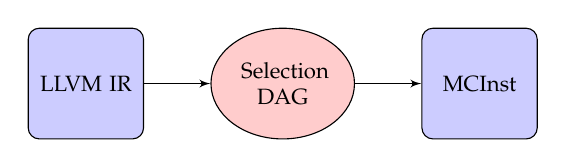
\begin{tikzpicture}[node distance = 2cm, auto]
\tikzstyle{every node}=[font=\footnotesize]
    % Düğümleri yerleştir
    \node [block] (init) {LLVM IR};
    \node [cloud, right of=init,node distance=2.5cm] (ast) {Selection DAG};
    \node [block, right of=ast,node distance=2.5cm] (llvmir) {MCInst};
    % Kenarları çiz
    \path [line] (init) -- (ast);
    \path [line] (ast) -- (llvmir);

   
\end{tikzpicture}
\end{center}
\end{frame}

\begin{frame}{LLVM IR ile Desen Eşleştirme}
Döndürme işlemi "ROTR", IR seviyesinde LLVM IR'de eşleştirilir.
    \begin{itemize}
        \item LLVM IR'de desen eşleştirme, bir içsel fonksiyonunun (intrinsic function) tanımını gerektirir.
        \item İçsel fonksiyon, desene göre optimizasyon geçişlerinde eşleştirilir.
        \item Eşleştirilen özdeşimler arka uca aktarılır ve yeni talimat yayınlanır.
    \end{itemize}
    LLVM IR'de desen eşleştirme daha esnek olabilir, ancak uygulamak daha karmaşık olabilir.
\end{frame}

\begin{frame}{MCInst ile Desen Eşleştirme}
SelectionDAG'den daha düşük bir seviye olan MCInst, talimatlar hakkında daha fazla ayrıntı gerektiğinde kullanılabilir.

"SH1ADD", materyalize edilmiş sabitlerin eşleştirilmesiyle LLVM'de uygulanmıştır. Sabitlerin farklı temsilleri olabilir ve belirli bir sabite ihtiyaç duyulursa, MCInst o sabiti eşleştirmek için daha fazla kontrol sağlar.
\end{frame}

\section{Conclusion}
\begin{frame}{Sonuç}
    Bulgularımız, özel talimat tasarımının kritik bir görev olduğunu göstermektedir. RISC-V standart uzantıları göz önünde bulundurulmalı ve analiz edilmelidir. Talimatlar, hem donanımı hem de yazılımı göz önünde bulundurarak tasarlanmalıdır.

    Desenler daha büyük hale geldikçe veya yüksek seviyeli bilgiler içerdikçe, orta uç gibi farklı derleyici aşamaları da göz önünde bulundurulmalıdır.

    Bu çalışma, okuyucunun bir derleyiciye herhangi bir özel talimat ekleme süreci hakkında sezgi sahibi olacağı çeşitli desen eşleştirme şemaları ve örnek uygulamaları sunmaktadır.
\end{frame}

\end{document} 
